\documentclass[13.5pt,aspecratio=169, xcolor=dvipsnames]{beamer}
\usepackage{graphicx} % Required for inserting images
\usepackage{subcaption}
\usepackage{amsfonts}
\usepackage{amsmath}
\usepackage{amssymb}
\usepackage{physics}
\usepackage{bm}
\usepackage{physics}
\usepackage{booktabs}
\usepackage{setspace}
\usepackage{xcolor}
\usepackage{wrapfig,lipsum}
\usetheme{Madrid}
\useinnertheme{circles}

\DeclareMathOperator*{\argmax}{arg\,max}
\DeclareMathOperator*{\argmin}{arg\,min}
\graphicspath{{Images/}{./}} 
\usetheme{Copenhagen}
\definecolor{UBCblue}{rgb}{0.04706, 0.13725, 0.26667} 
\usecolortheme[named=UBCblue]{structure}
%\usecolortheme{beaver}
\title{Spot The Differences Between Two Images}
\author[CS231]{\textit{Le Gia Khang \\ Le Duy Khang \\ Nguyen Hoang Tan }\\ \bigskip \textbf{CS231: Introduction to Computer Vision}}
\date{\today}
\definecolor{mylightgreencolor}{RGB}{144, 238, 144}
\definecolor{mylightredcolor}{RGB}{255, 204, 203}
\setbeamertemplate{navigation symbols}{}
\setbeamertemplate{headline}{}
\setbeamercolor{huge text}{fg=white}
\setbeamertemplate{footline}{
    \leavevmode%
    \hbox{%
        \begin{beamercolorbox}[wd=.2\paperwidth,ht=2.25ex,dp=1ex,center]{author in head/foot}%
            \usebeamerfont{author in head/foot}\insertshortauthor
        \end{beamercolorbox}%
        \begin{beamercolorbox}[wd=.6\paperwidth,ht=2.25ex,dp=1ex,center]{title in head/foot}%
            \usebeamerfont{title in head/foot}\insertshorttitle
        \end{beamercolorbox}%
        \begin{beamercolorbox}[wd=.2\paperwidth,ht=2.25ex,dp=1ex,right]{date in head/foot}%
            \insertframenumber{} / \inserttotalframenumber\hspace*{2ex} 
        \end{beamercolorbox}%
    }%
    \vskip0pt%
}

\begin{document}
\maketitle

% \begin{frame}
% 	\frametitle{Table of Contents} % Slide title, remove this command for no title
% 	\tableofcontents[subsectionstyle=hide]
% \end{frame}
%-------------------------------------------------------------------%


\begin{frame}
    \doublespacing
        \frametitle{Presentation Overview} % Slide title, remove this command for no title
        
        \tableofcontents % Output the table of contents (all sections on one slide)
        %\tableofcontents[pausesections] % Output the table of contents (break sections up across separate slides)
\end{frame}
    
    %----------------------------------------------------------------------------------------
    %	PRESENTATION BODY SLIDES
    %----------------------------------------------------------------------------------------
    
    \section{Problem Statement} % Sections are added in order to organize your presentation into discrete blocks, all sections and subsections are automatically output to the table of contents as an overview of the talk but NOT output in the presentation as separate slides
    %------------------------------------------------
    \begin{frame}
        \doublespacing
            \frametitle{Presentation Overview} % Slide title, remove this command for no title
            
            \tableofcontents[currentsection] % Output the table of contents (all sections on one slide)
            %\tableofcontents[pausesections] % Output the table of contents (break sections up across separate slides)
    \end{frame}

%-------------------------------------------------------------------%

\subsection{Why it Matters}
\begin{frame}
    \onehalfspacing
        \frametitle{Why it Matters}
        
        \begin{minipage}{0.55\textwidth}
            \begin{minipage}{0.9\textwidth}
            \begin{block}{Applications}
                Detecting changes is a natural computer
                vision task:
                \begin{itemize}
                    \item The “spot-the-difference” game
                    \item Facility monitoring
                    \item Medical imaging
                    \item Satellite surveillance
                    \item Counterfeit detection
                \end{itemize}
                ... and many more.
            \end{block}
        \end{minipage}
        \end{minipage}
        \begin{minipage}{0.4\textwidth}
            \begin{figure}[h]
            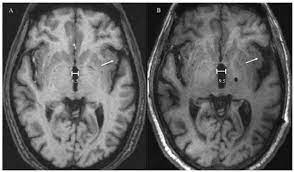
\includegraphics[scale=0.55]{Medical_Imaging.jpg}
            \begin{center}
            \hspace{1em} Comparison of two MRI \\ \hspace{1em} scans over 10-year period. 
            \end{center}
            \end{figure}
        \end{minipage}
    \end{frame}
    
    %--------------------------------------------------
    \subsection{Input and Output Analysis}

    \begin{frame}
    \onehalfspacing
        \frametitle{Input and Output Analysis}
            \begin{block}{\begin{center}Input\end{center}}
                \vspace{1em}
                \begin{center}Pair of images need to compare \hphantom{with bounding boxes to indicate
                    areas of distinction
                    }\end{center}
                
                \begin{figure}
                    \centering
                    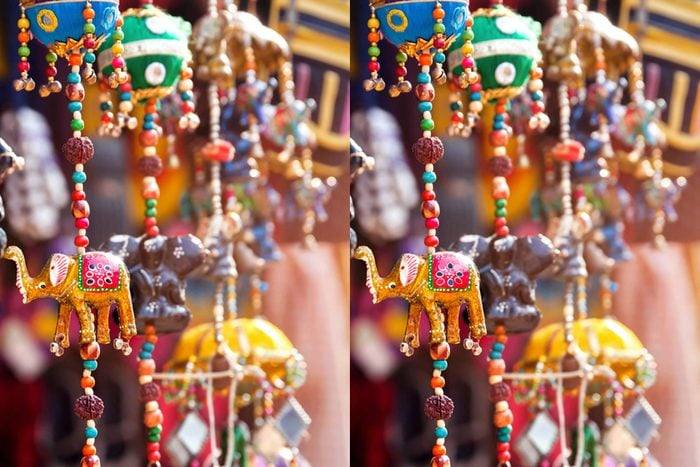
\includegraphics[scale=0.3]{Example/07_full.jpg}
                \end{figure}
            \end{block}
    \end{frame}
    
    
    %------------------------------------------------
    \begin{frame}
        \onehalfspacing
            \frametitle{Input and Output Analysis}
                \begin{block}{\begin{center}Output\end{center}}
                    \vspace{1em}
                    \begin{center}The provided images are marked with bounding boxes \\ to indicate areas of distinction\end{center}
                    
                    \begin{figure}
                        \centering
                        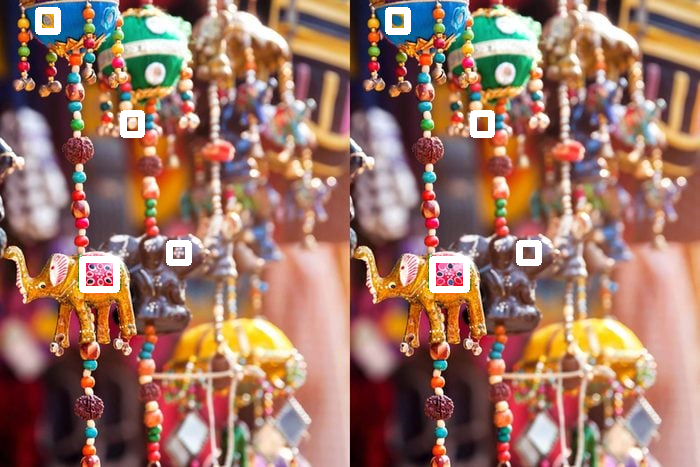
\includegraphics[scale=0.3]{Example/7_res_full.png}
                    \end{figure}
                \end{block}
        \end{frame}
    
    %------------------------------------------------
    
    \subsection{Examples}

    \begin{frame}
    \onehalfspacing
        \frametitle{Examples: Input}
        \hspace{1em}
        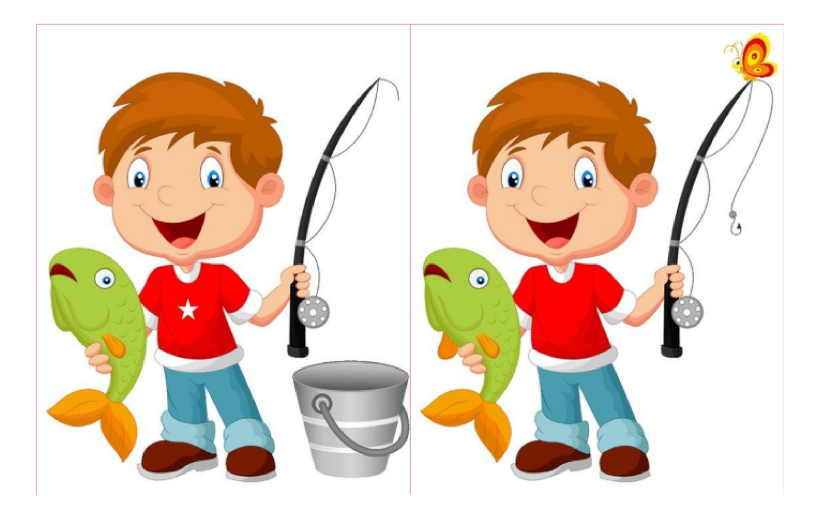
\includegraphics[scale=0.5]{Example/Fishing_boy.png}
    \end{frame}
    %------------------------------------------------

    \begin{frame}
        \onehalfspacing
            \frametitle{Examples: Input}
            \begin{figure}[h]
            \centering
            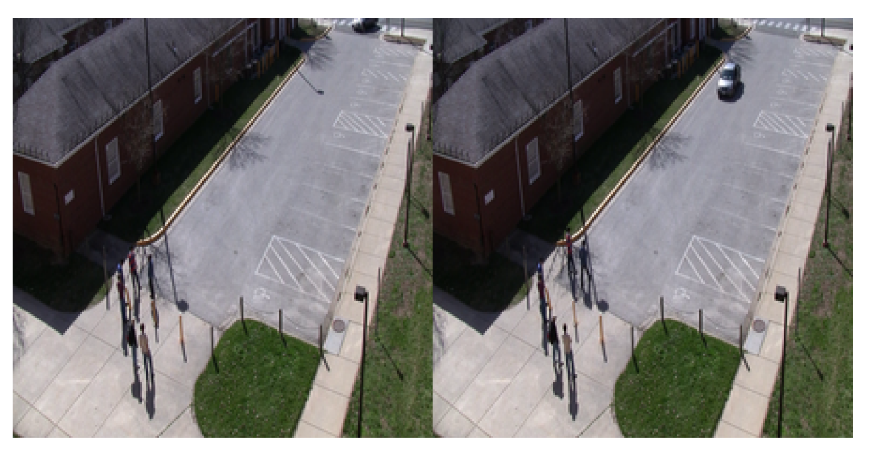
\includegraphics[scale=0.5]{Example/Camera_1.png}
            \end{figure}
        \end{frame}
        %------------------------------------------------

        \begin{frame}
            \onehalfspacing
                \frametitle{Examples: Input}
                \begin{figure}[h]
                \centering
                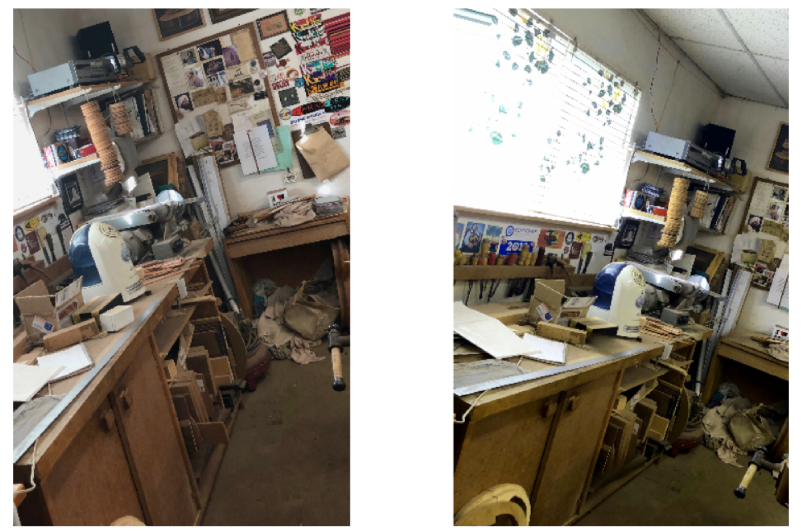
\includegraphics[scale=0.5]{Example/Example_1.png}
                \end{figure}
            \end{frame}
            %------------------------------------------------
    

            \begin{frame}
            \onehalfspacing
                \frametitle{Examples: Output}
                \hspace{1em}
                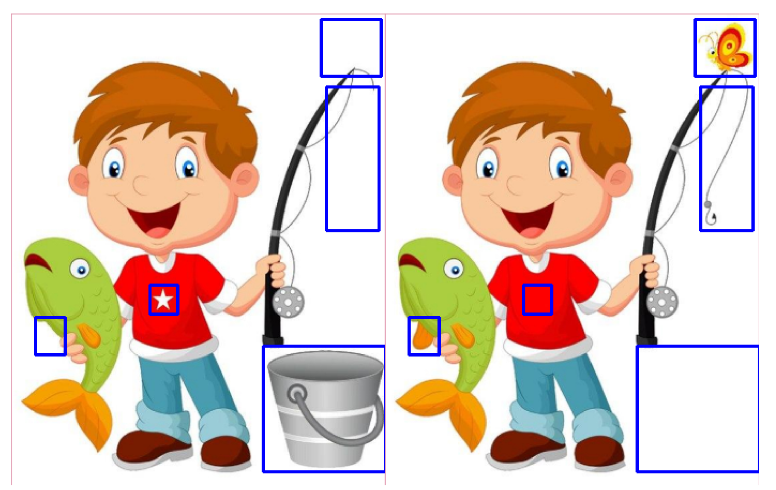
\includegraphics[scale=0.5]{Example/Fishing_boy_bb.png}
            \end{frame}
            %------------------------------------------------
        
            \begin{frame}
                \onehalfspacing
                    \frametitle{Examples: Output}
                    \begin{figure}[h]
                    \centering
                    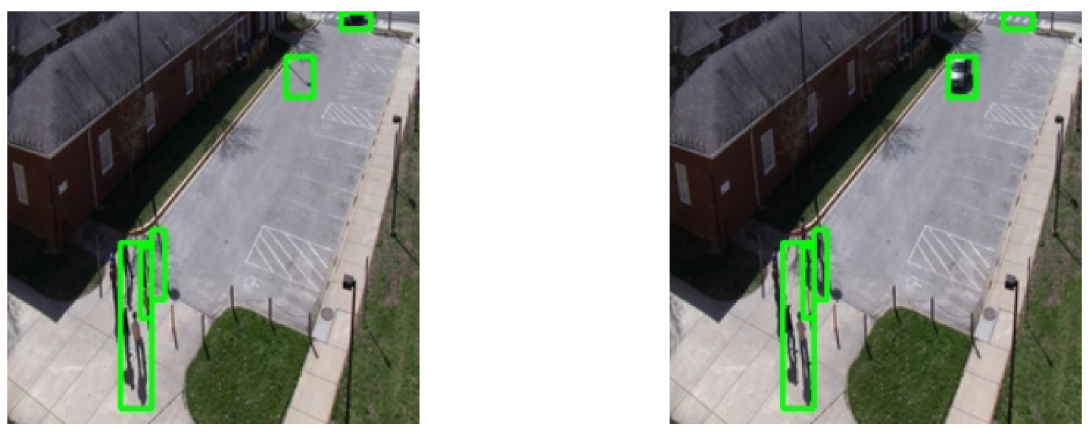
\includegraphics[scale=0.4]{Example/Camera_1_bb.png}
                    \end{figure}
                \end{frame}
                %------------------------------------------------
        
                \begin{frame}
                    \onehalfspacing
                        \frametitle{Examples: Output}
                        \begin{figure}[h]
                        \centering
                        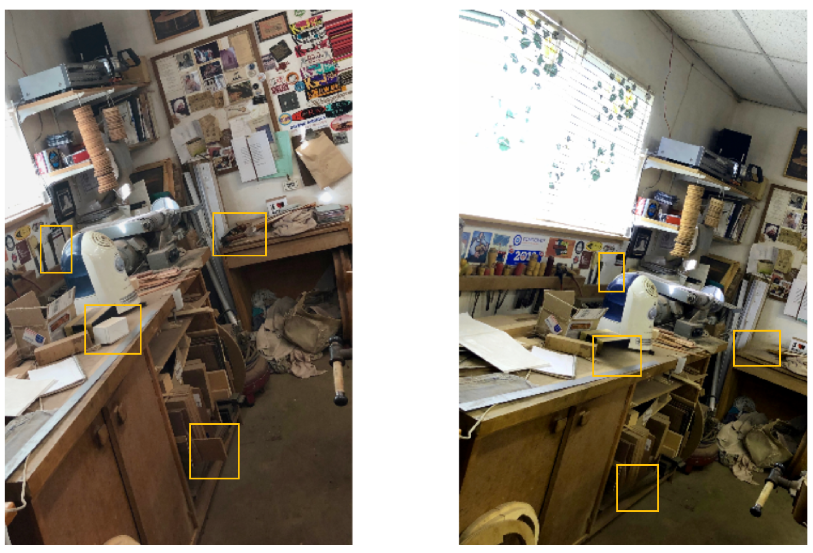
\includegraphics[scale=0.5]{Example/Example_1_bb.png}
                        \end{figure}
                    \end{frame}
                    %------------------------------------------------
            

    
\section{Methodology} % Sections are added in order to organize your presentation into discrete blocks, all sections and subsections are automatically output to the table of contents as an overview of the talk but NOT output in the presentation as separate slides
\begin{frame}
	\frametitle{Presentation Overview} % Slide title, remove this command for no title
	\tableofcontents[currentsection]
\end{frame}


\subsection{Pixel-Wise Comparison}
\begin{frame}
    \frametitle{Presentation Overview}
    \tableofcontents[currentsubsection, sectionstyle=show/shaded, subsectionstyle=show/shaded]
\end{frame}

%------------------------------------------------
\begin{frame}
    \onehalfspacing
        \frametitle{Pixel-Wise}
        
        \begin{block}{Pixel-Wise Comparison}
            Compare the input image pair by first detecting which \textbf{pixels} have \textbf{changed} between the first and second image and then \textbf{segmenting} those pixels into \textbf{clusters} that \textit{approximately} represent the objects that have changed.

        \end{block}

        Or, in short:
        \begin{enumerate}
            \item Detect pixels that have changed.
            \item Perform clustering on those pixels.
        \end{enumerate}
      
\end{frame}
    
%------------------------------------------------

\begin{frame}
    \onehalfspacing
        \frametitle{Pixel-Wise: Detect changes in pixels}
        
        \begin{minipage}{0.9\textwidth}
            \begin{block}{}
                \textbf{Base approach}: pixel changes when its value is not the same.
            \end{block}
        \end{minipage}
        
        \bigskip

        Well, it works fine… with digital changes (e.g. photoshop,...)

        \bigskip

        \begin{figure}[h]
            \centering
            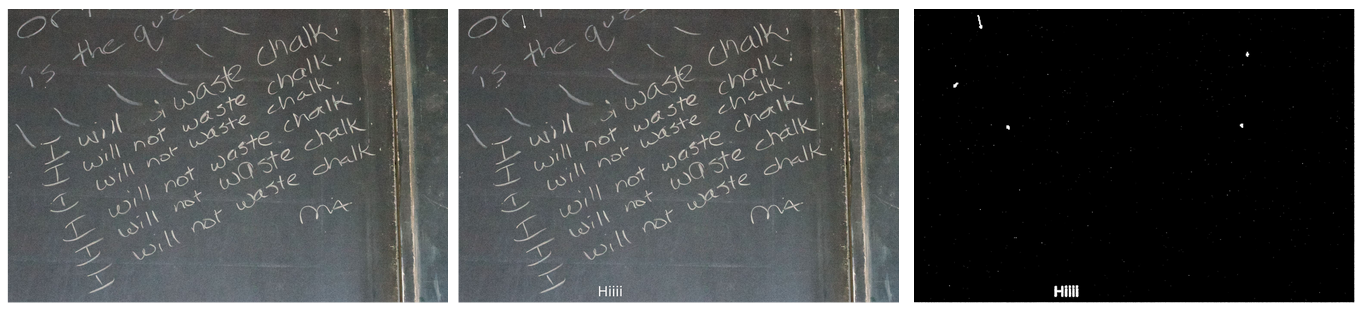
\includegraphics[width=\linewidth]{Pixel_wise_1.png}
        \end{figure}
      
\end{frame}
    
%------------------------------------------------

\begin{frame}
    \onehalfspacing
        \frametitle{Pixel-Wise: Detect changes in pixels}
        
        
        
        But fails horribly with non-digital changes (e.g. camera’s noises, environmental changes, …)


        \bigskip

        \begin{figure}[h]
            \centering
            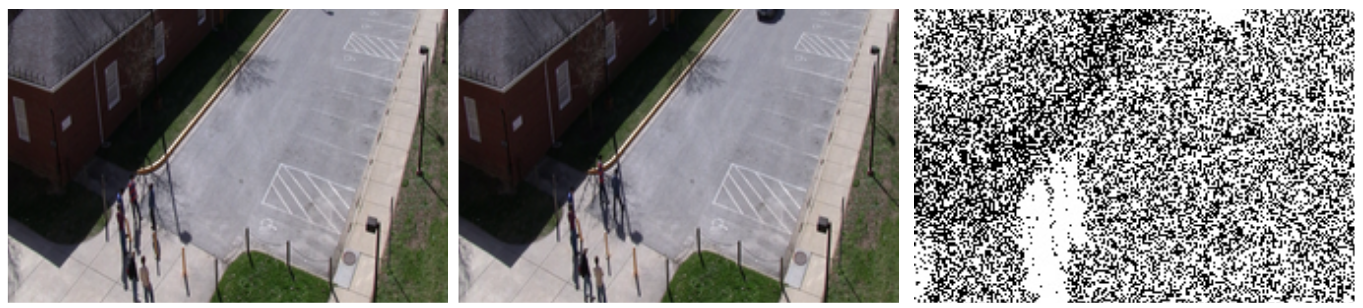
\includegraphics[width=\linewidth]{Pixel_wise_2.png}
        \end{figure}
      
\end{frame}
    
%------------------------------------------------

\begin{frame}
    \onehalfspacing
        \frametitle{Pixel-Wise: Detect changes in pixels}
        
        
        
        So, \textbf{some changes are tolerable}. Hence, we will need to compute the \textbf{distance} between two pixels and compare that against a \textbf{threshold} value.

        \bigskip

        \begin{figure}[h]
            \centering
            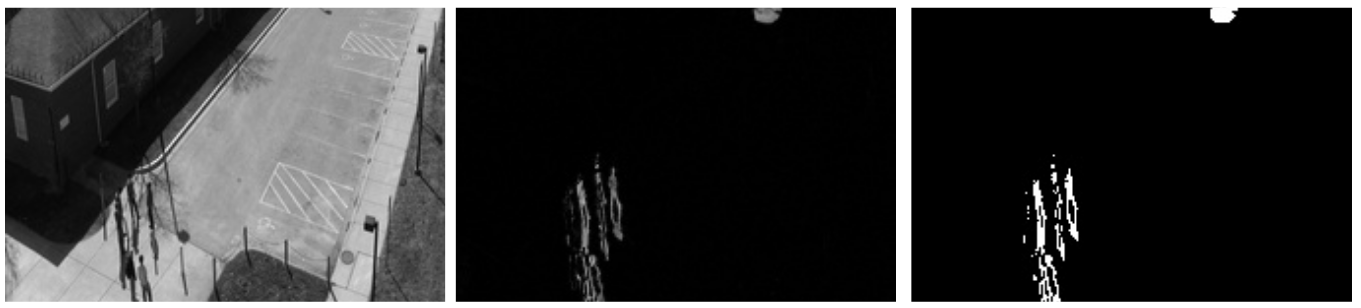
\includegraphics[width=\linewidth]{Pixel_wise_threshold.png}
        \end{figure}

        \bigskip

        The most popular method of computing that distance is to compute the difference between the two pixels’ \textbf{luminosity} (convert images into grayscale and then compare its values).

      
\end{frame}
    
%------------------------------------------------

\begin{frame}
    \onehalfspacing
        \frametitle{Pixel-Wise: Detect changes in pixels}
        
        
        
        However, some colours have similar \textbf{grayscale representation} despite not being the same color. 

        \bigskip

        \begin{figure}
            \begin{subfigure}{0.5\textwidth}
              \centering
              
\includegraphics[width=\linewidth]{RGB_color.png}
              \captionsetup{labelformat=empty}
              \caption{RGB(0, 0, 255) and RGB(0, 48, 0)}
            \end{subfigure}%
            \begin{subfigure}{0.5\textwidth}
              \centering
              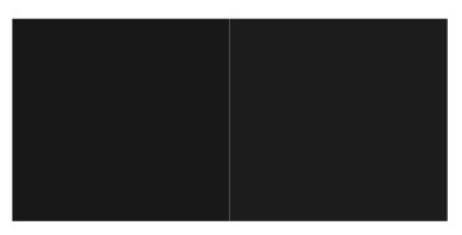
\includegraphics[width=0.985\linewidth]{RGB_color_grayscale.png}
              \captionsetup{labelformat=empty}
              \caption{Convert to \textbf{grayscale}}
            \end{subfigure}
            \captionsetup{labelformat=empty}
        \end{figure}

        \bigskip

        

      
\end{frame}
    
%------------------------------------------------

\begin{frame}
    \onehalfspacing
        \frametitle{Pixel-Wise: Detect changes in pixels}
        
        
        \begin{minipage}{0.53\textwidth}
            \begin{block}{}
                Distance between colours $C_1$ and $C_2$:
            \end{block}
        \end{minipage}
        


        \bigskip

        \begin{figure}
           \centering
           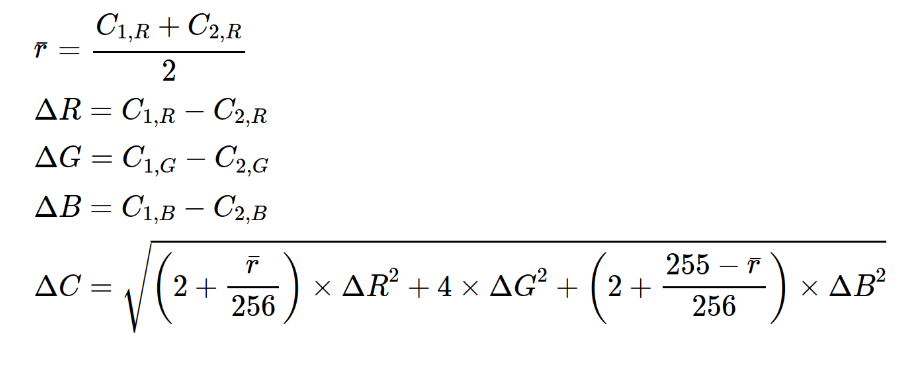
\includegraphics[width=\linewidth]{color_distance.png}
        \end{figure}

        \bigskip

      
\end{frame}
    
%------------------------------------------------

\begin{frame}
    \onehalfspacing
        \frametitle{Pixel-Wise: Detect changes in pixels}
        
        

            \begin{figure}
                \centering
                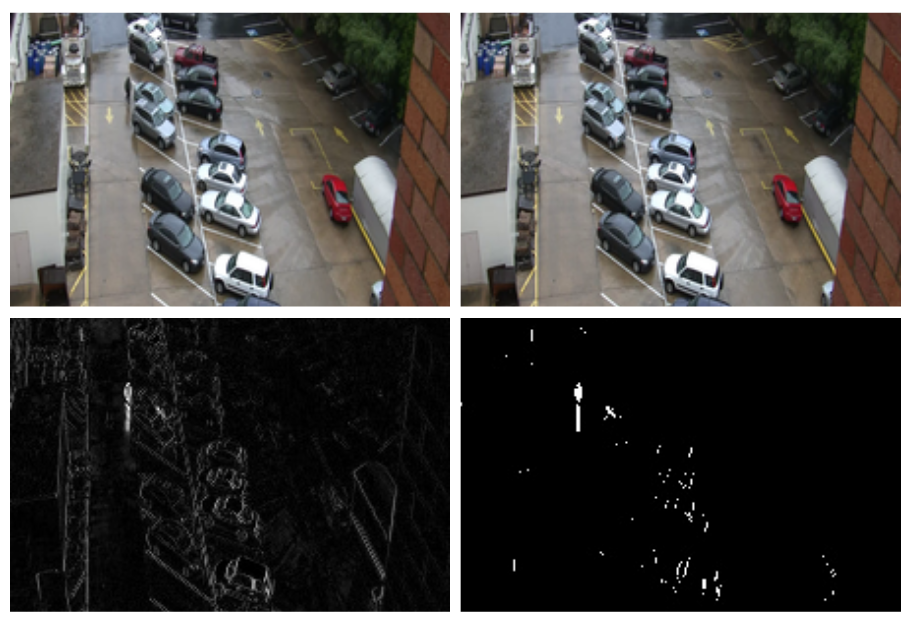
\includegraphics[width=0.85\linewidth]{Pixel_wise_color_distance_result.png}
                \caption{ Result after applying the colour distance function}
             \end{figure}
        
      
\end{frame}
    
%------------------------------------------------

\begin{frame}
    \onehalfspacing
        \frametitle{Pixelwise: Clustering
        }
        \begin{block}{}
            As we only care about \textbf{objects} that have changed not changed pixels, we have to group those pixels \textbf{into clusters} that approximate those objects.
        \end{block}


            \begin{figure}
                \centering
                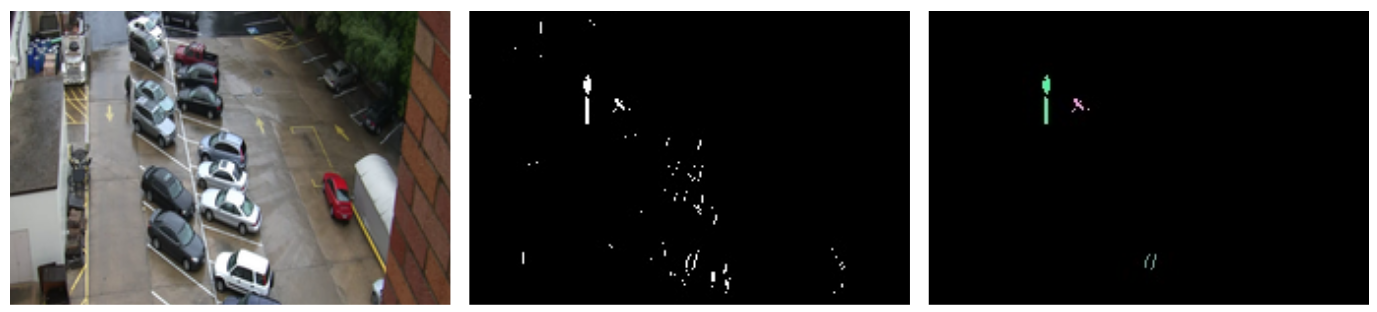
\includegraphics[width=\linewidth]{pixel_wise_clustering.png}
             \end{figure}


        And, due to the characteristics of those pixels (denser area is more likely to be an object than noises) \textbf{density based clustering algorithms} like \textit{DBScan} will perform well.
        
      
\end{frame}
    
%------------------------------------------------

\begin{frame}
    \onehalfspacing
        \frametitle{Pixelwise: Clustering
        }
        \begin{minipage}{0.8\textwidth}
        \begin{block}{}
            Finally. encapsulate those clusters with bounding boxes.
        \end{block}
    \end{minipage}

    \bigskip

            \begin{figure}
                \centering
                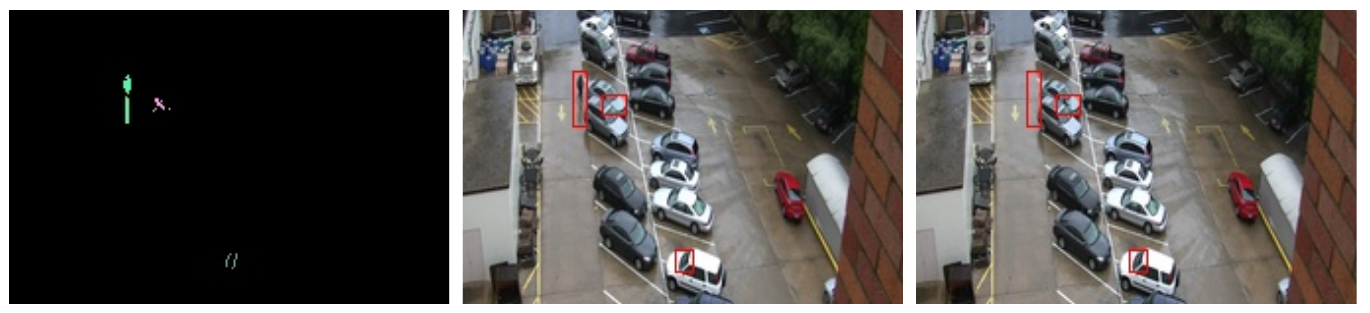
\includegraphics[width=\linewidth]{pixel_wise_clusters_with_bounding_boxes.png}
             \end{figure}
      
\end{frame}
    
%------------------------------------------------


\begin{frame}
    \onehalfspacing
        \frametitle{Pixel-wise optional: Remove non-interesting clusters
        }
        \begin{block}{}
            In images from a surveillance video, a lot of unnecessary changes are detected like slight movement, reflective area, …
        \end{block}

        These clusters can be reduced by using a simple scoring system:

        \hspace{4em}\rule{0.7\textwidth}{0.4pt}
        \vspace{-0.5em}
        {\small
        \begin{center}
            $ number\_of\_changed\_pixels + height\_of\_cluster \times 2 + width\_of\_cluster \geq threshold $
        \end{center}
        }
        \vspace{-1em}
        \hspace{4em}\rule{0.7\textwidth}{0.4pt}


            \begin{figure}
                \centering
                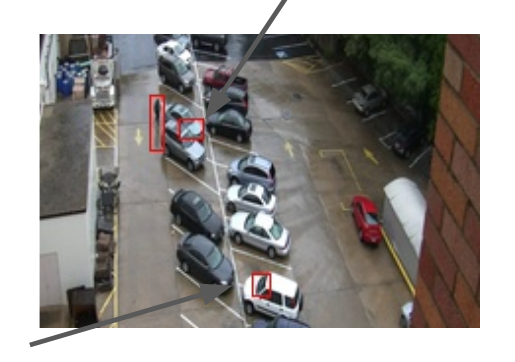
\includegraphics[width=0.55\linewidth]{Remove_non_interesting_clusters.png}
             \end{figure}
      
\end{frame}
    
%------------------------------------------------


\subsection{Structural similarity index (SSIM)}

\begin{frame}
    \frametitle{Presentation Overview}
    \tableofcontents[currentsubsection, sectionstyle=show/shaded, subsectionstyle=show/shaded]
\end{frame}

\begin{frame}
    \onehalfspacing
        \frametitle{Structural similarity index (SSIM)}
        
        \begin{block}{Structural similarity index (SSIM)}
            SSIM is used as a metric to measure the similarity between two given images which is a value between -1 and +1.
            \begin{itemize}
            \item Designed to mimic human perception in evaluating image quality.
            \item It takes into account \textit{luminance, contrast}, and \textit{structure}.
            \end{itemize}
        \end{block}

        \begin{figure}[h]
            \centering
            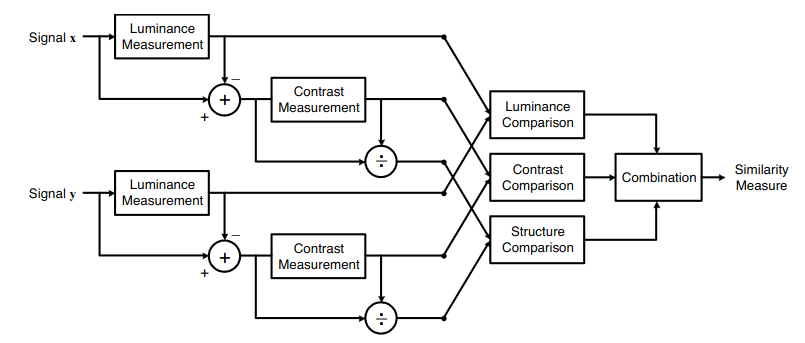
\includegraphics[width=0.9\linewidth]{SSIM.png}
            \caption{Diagram of the structural similarity (SSIM) measurement system}
        \end{figure}
      
\end{frame}
    
%------------------------------------------------

\begin{frame}
    \onehalfspacing
        \frametitle{SSIM: Luminance}
        
        \textbf{Luminance} is measured by \textbf{averaging} over all the pixel values. Its denoted by $\mu$ and the formula is given below:
        \smallskip
        {\Large
        \begin{center}
            $ \mu_x = \dfrac{1}{N} \sum_{i=1}^{N} x_i$
        \end{center}
        }

        \begin{block}{The luminance comparison function $\ell(x,y)$}
            {\Large
            \begin{center}
                $ \ell(x,y) = \dfrac{2\mu_{\textbf{x}} \mu_{\textbf{y}} + C_1}{\mu^2_{\textbf{x}} + \mu^2_{\textbf{y}} + C_1} $
            \end{center}
            }
            \hspace{8em}\rule{0.5\textwidth}{0.4pt}
            \begin{itemize}
                \item {\Large $\mu_{\textbf{x}}, \hspace{0.2em} \mu_{\textbf{y}}$}: Mean luminance of the first and second image.
                \item $C_1 = (K_1 L)^2$: where L = 255 for 8-bit component images.
                \item $K_1 \ll 1$: Default value is $.01$
            \end{itemize}
        \end{block}
        
        
      
\end{frame}
    
%------------------------------------------------

\begin{frame}
    \onehalfspacing
        \frametitle{SSIM: Contrast}
        
        \textbf{Contrast} is measured by taking the standard deviation (square root of variance) of all the pixel values. It is denoted by $\sigma$
        \smallskip
        {\Large
        \begin{center}
            $ \sigma_x = \sqrt{\frac{1}{N-1} \sum_{i=1}^{N} (x_i - \mu_x)^2} $
        \end{center}
        }

        \begin{block}{The luminance comparison function $\c(x,y)$}
            {\Large
            \begin{center}
                $ c(x,y) = \dfrac{2\sigma_{\textbf{x}} \sigma_{\textbf{y}} + C_2}{\sigma^2_{\textbf{x}} + \sigma^2_{\textbf{y}} + C_2} $
            \end{center}
            }
            \hspace{8em}\rule{0.5\textwidth}{0.4pt}
            \begin{itemize}
                \item {\Large$\sigma_{\textbf{x}}, \hspace{0.2em} \sigma_{\textbf{y}}$}: The standard deviation of pixel values
                \item $C_2 = (K_2 L)^2$: where L = 255 for 8-bit component images.
                \item $K_2 \ll 1$: Default value is $.03$
            \end{itemize}
        \end{block}
        
        
      
\end{frame}
    
%------------------------------------------------


\begin{frame}
    \onehalfspacing
        \frametitle{SSIM: Structure}
        
        The formula for covariance {\Large $\sigma_{xy}$} between $x$ and $y$ is given by:
        \smallskip
        {\Large
        \begin{center}
            $ \sigma_{xy} = \dfrac{1}{N-1} \sum_{i=1}^{N} (x_i - \mu_x)(y_i - \mu_y)
              $
        \end{center}
        }

        \begin{block}{Structure comparison function $s(x,y)$}
            {\Large
            \begin{center}
                $ s(x,y) = \dfrac{\sigma_{\textbf{xy}} + C_3}{\sigma_{\textbf{x}} \sigma_{\textbf{y}} + C_3} $
            \end{center}
            }
            \hspace{8em}\rule{0.5\textwidth}{0.4pt}
            \begin{itemize}
                \item {\Large $\sigma_{\textbf{xy}}$}: The covariance between $x$ and $y$.
                \item $C_3 = C_2 / 2$.
            \end{itemize}
        \end{block}
        
        
      
\end{frame}
    
%------------------------------------------------

\begin{frame}
    \onehalfspacing
        \frametitle{The SSIM score}
        
        And finally, the SSIM score is given by,
        \begin{figure}
            \centering
            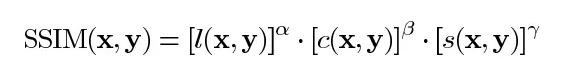
\includegraphics[width=0.8\linewidth]{SSIM_Formula.png}
        \end{figure}
            \begin{block}{}
                Where $\alpha > 0, \beta > 0, \gamma > 0$ denote the importance of each of the metrics. 
            \end{block}

        To simplify the expression, if we assume, $\alpha = \beta = \gamma = 1$, we can get,
        \begin{figure}
            \centering
            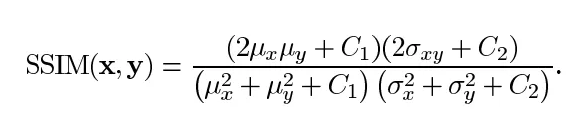
\includegraphics[width=0.8\linewidth]{SSIM_Formula_Simp.png}
        \end{figure}
        
\end{frame}
    
%------------------------------------------------

\begin{frame}
    \onehalfspacing
        \frametitle{Mean Structural Similarity Index}
        
        Instead of applying the above metrics globally, it’s better to apply the metrics regionally
        \begin{block}{Mean Structural Similarity Index (MSSIM)}
            For image quality assessment, it is useful to apply the SSIM index locally rather than globally.
            \begin{itemize}
                \item Image statistical features are usually highly spatially nonstationary.
                \item Image distortions, which may or may not depend on the local image statistics, may also be space-variant.
                \item Only a local area in the image can be perceived with high resolution by the human observer at one time instance 
            \end{itemize}
        \end{block}
\end{frame}
    
%------------------------------------------------


\begin{frame}
    \onehalfspacing
        \frametitle{Mean Structural Similarity Index}
        
        
        \begin{block}{Gaussian Weighing}
            We use an 11x11 circular-symmetric Gaussian Weighing function 
            \begin{itemize}
                \item Moves pixel-by-pixel over the entire image.
                \item At each step, the local statistics and SSIM index are calculated within the local window. 
            \end{itemize}
        \end{block}
        \begin{minipage}{0.6\textwidth}
            \begin{figure}
                \centering
                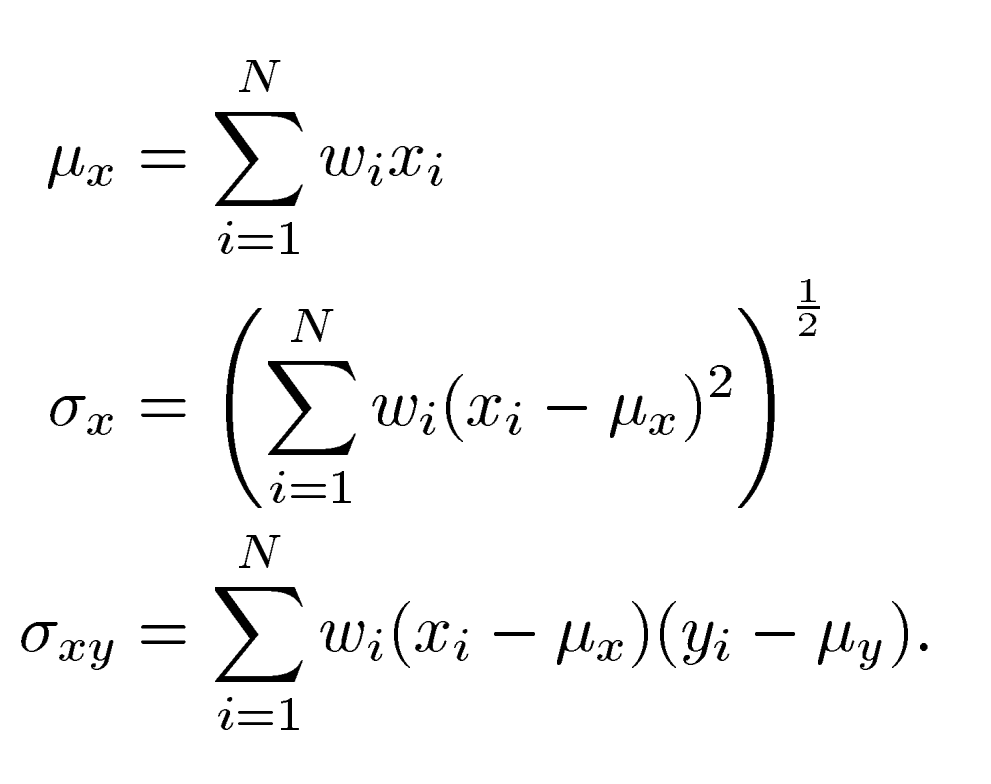
\includegraphics[width=0.9\linewidth]{gaussian_weighting.png}
            \end{figure}
        \end{minipage}
        \begin{minipage}{0.39\textwidth}
            \begin{center}
                Where $w_i$ is the gaussian weighting function.
            \end{center}
        \end{minipage}
       
\end{frame}
    
%------------------------------------------------


\begin{frame}
    \onehalfspacing
        \frametitle{Mean Structural Similarity Index}
        
        Once computations are performed all over the image, we simply take the \textit{mean of all the local SSIM values} and arrive at the global SSIM value.

        \begin{figure}[h]
            \centering
            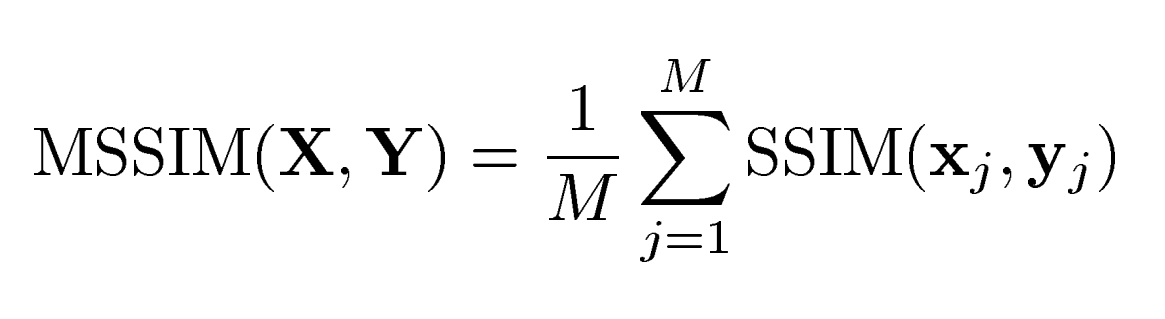
\includegraphics[width=0.7\linewidth]{MSSIM_formula.png}
        \end{figure}
       
\end{frame}
    
%------------------------------------------------


\begin{frame}
    \onehalfspacing
        \frametitle{SSIM: Examples}
        
        \begin{figure}
            \centering
            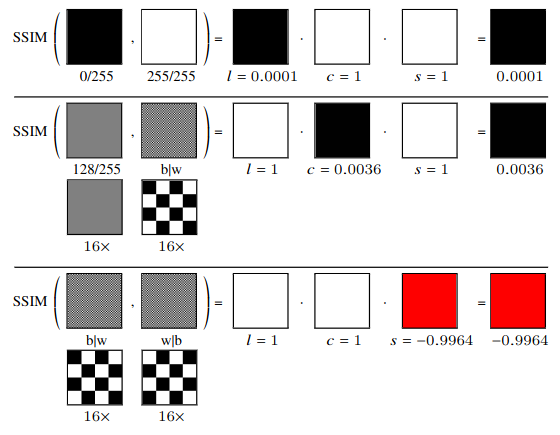
\includegraphics[width=0.8\linewidth]{SSIM_Example_1.png}
        \end{figure}
        
       
\end{frame}
    
%------------------------------------------------

\begin{frame}
    \onehalfspacing
        \frametitle{SSIM: Examples}
        
        \begin{minipage}{0.6\textwidth}
            \begin{figure}
                \centering
                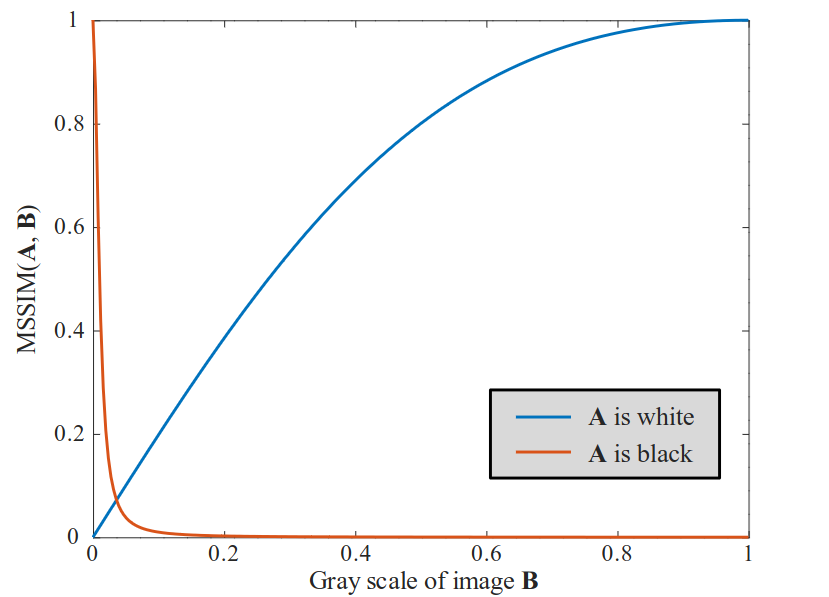
\includegraphics[width=\linewidth]{MSSIM_Fig_1.png}
                \captionsetup{labelformat=empty}
                \caption{{\tiny MSSIM as a function of an increasingly brighter, constant-valued
                image, B, against a black image (orange curve) and a white image (blue curve).}}
            \end{figure}
        \end{minipage}
        \begin{minipage}{0.39\textwidth}
            \begin{figure}
                \centering
                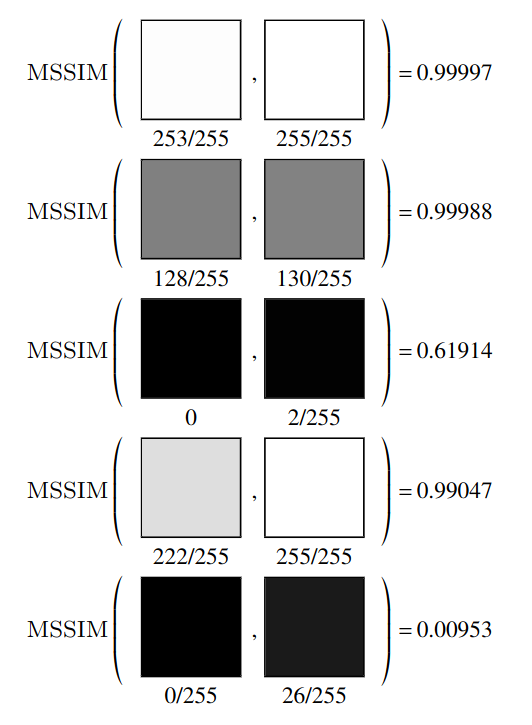
\includegraphics[width=\linewidth]{MSSIM_Fig_2.png}
                \captionsetup{labelformat=empty}
                \caption{{\tiny MSSIM behavior for constant grayscale images. }}
            \end{figure}
        \end{minipage}
        
        
       
\end{frame}
    
%------------------------------------------------
\subsection{Siamese Network}

\begin{frame}
    \frametitle{Presentation Overview}
    \tableofcontents[currentsubsection, sectionstyle=show/shaded, subsectionstyle=show/shaded]
\end{frame}

%------------------------------------------------

\begin{frame}
    \onehalfspacing
        \frametitle{Siamese Network}
        Proposed in the article "The Change You Want To See" accepted at the IEEE/CVF Winter Conference on Application of Computer Vision 2023.
        \bigskip
        \begin{figure}
            \begin{subfigure}{0.5\textwidth}
              \centering
              \includegraphics[width=0.7\linewidth]{Regav.png}
              \captionsetup{labelformat=empty}
              \caption{Ragav Sachdeva}
              \label{fig:subfig1}
            \end{subfigure}%
            \begin{subfigure}{0.5\textwidth}
              \centering
              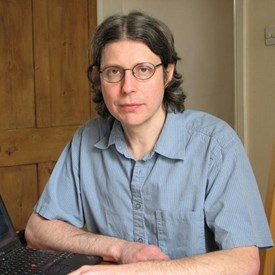
\includegraphics[width=0.7\linewidth]{Zisserman.jpg}
              \captionsetup{labelformat=empty}
              \caption{Andrew Zisserman}
              \label{fig:subfig2}
            \end{subfigure}
            \captionsetup{labelformat=empty}
            \caption{Visual Geometry Group at the University of Oxford}
            \label{fig:overall}
        \end{figure}
      
\end{frame}
    
%------------------------------------------------

\begin{frame}
    \onehalfspacing
        \frametitle{Siamese Network: Overview}
        \begin{itemize}
            \item Enable “object-level” change prediction and simplify counting the number of changes between two images.
            \item Use an architecture that operates on two images with
            geometric (scale, rotation,..) and photometric changes.
            \item Designed to be
            class-agnostic, it can detect changes irrespective of
            the object classes involved. 
        \end{itemize}
        
        \begin{figure}
            \centering
            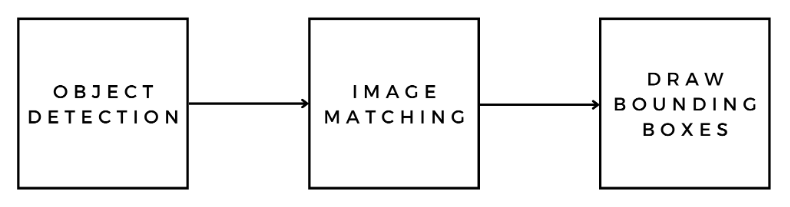
\includegraphics[scale=0.5]{Siamese_network_1.png}
        \end{figure}
        
\end{frame}

%------------------------------------------------


\begin{frame}
    \onehalfspacing
        \frametitle{Model Architecture Overview}
        \begin{figure}
            \centering
            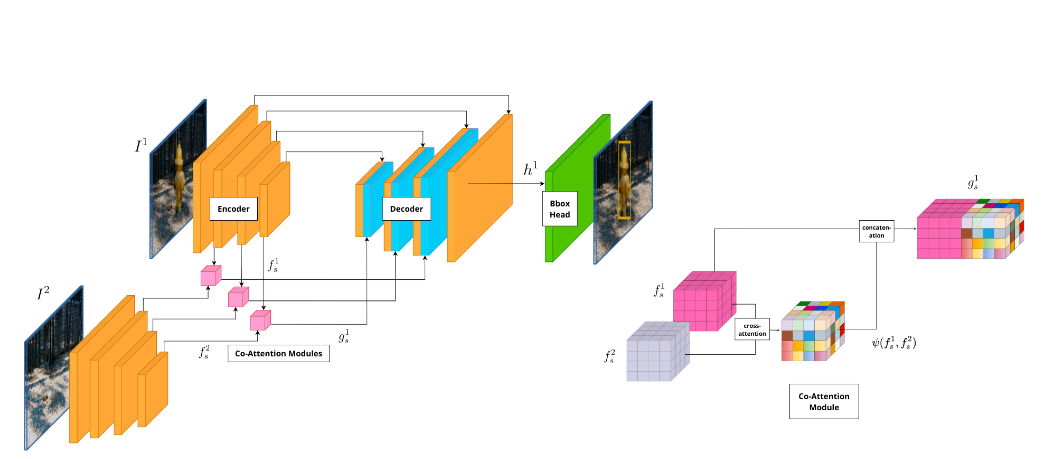
\includegraphics[width=\linewidth]{Siamese_network_architecture.png}
            \caption{\textbf{Architecture}: Utilizing a dual-image encoder, feature maps $(f^s_1, f^s_2)$ are generated. A co-attention module aligns and conditions these maps $(g^s_1, g^s_2)$. Subsequently, a U-Net decoder processes the original and conditioned maps to yield final feature maps $(h_1, h_2)$. The bounding box detector head employs $h_1$ and $h_2$ to generate bounding boxes for images $I_1$ and $I_2$, respectively}
        \end{figure}
        
\end{frame}

%------------------------------------------------



\begin{frame}
\onehalfspacing
	\frametitle{Siamese Network: Overview}
    \begin{block}{Siamese Network}
        A type of neural network architecture designed for tasks involving similarity or distance measurement between input pairs. 
        \begin{itemize}
            \item Consists of two identical subnetworks (or twins) that share the same set of weights and parameters.
            \item The name originates from Chang (left) and Eng Bunker (right).
        \end{itemize}
    \end{block}

    \begin{figure}
        \centering
        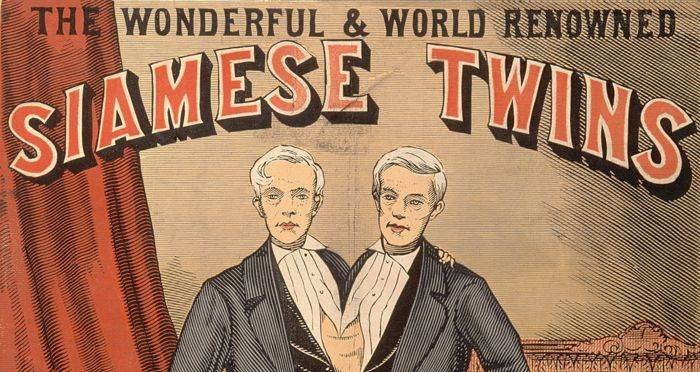
\includegraphics[scale=0.3]{Siamese_Twin.jpg}
    \end{figure}
\end{frame}

%------------------------------------------------
\begin{frame}
    \onehalfspacing
        \frametitle{Siamese Network: Architecture}
        
       \begin{itemize}
            \item Consists of two identical subnetworks.
            \item Extract feature vectors from both networks using a common set of convolutional and fully connected layers.
            \item Feature vectors from both networks are compared using a loss function $L$.
       \end{itemize}
       \begin{figure}
            \centering
            \includegraphics[scale=0.5]{Siamese_architecture.png}
       \end{figure}
        
\end{frame}
%------------------------------------------------
\begin{frame}
    \onehalfspacing
        \frametitle{U-Net Encoder-Decoder Network}
        U-Net is a type of convolutional neural network (CNN) architecture commonly used for image segmentation tasks.
        \begin{minipage}{0.55\textwidth}
            \begin{minipage}{0.95\textwidth}
            \begin{block}{Consists of an encoder-decoder structure:}
                \begin{itemize}
                    \item \textbf{Encoder:} capturing features from the input image. 
                    \item \textbf{Decoder:} upsampling and producing a segmented output.
                \end{itemize}
            \end{block}
        \end{minipage}
        \end{minipage}
        \begin{minipage}{0.35\textwidth}
            \begin{figure}[h]
                \centering
                \hspace{10em}
                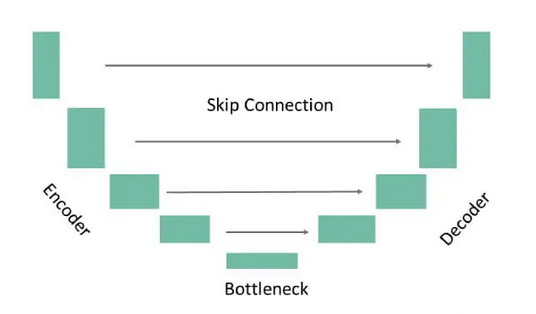
\includegraphics[scale=0.4]{U_net.png}
            \end{figure}
        \end{minipage}

        \vspace{2em}
        The authors employed \textbf{ResNet50} as the CNN for the encoder.
\end{frame}
%------------------------------------------------

\begin{frame}
    \onehalfspacing
        \frametitle{A UNet encoder-decoder with CoAM}
        
        \begin{block}{CoAM Attention Module}
            We wish to concatenate features from both images in order to condition the model on both input images.
            \begin{itemize}
                \item However, for a given spatial location, the
                relevant feature in the other image may not be at the same spatial location.
            \end{itemize}
            As a result, we use an
            attention mechanism to model long range dependencies.
        \end{block}
        \begin{figure}[h]
            \centering
            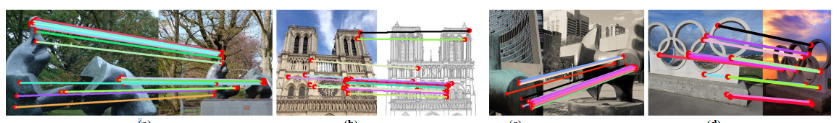
\includegraphics[width=\linewidth]{CoAM_model.png}
            \caption{Correspondences obtained with the CoAM model, which is augmented with an attention mechanism. }
        \end{figure}
\end{frame}
%------------------------------------------------

\begin{frame}
\onehalfspacing
	\frametitle{A UNet encoder-decoder with CoAM}
    \begin{figure}[h]
        \centering
        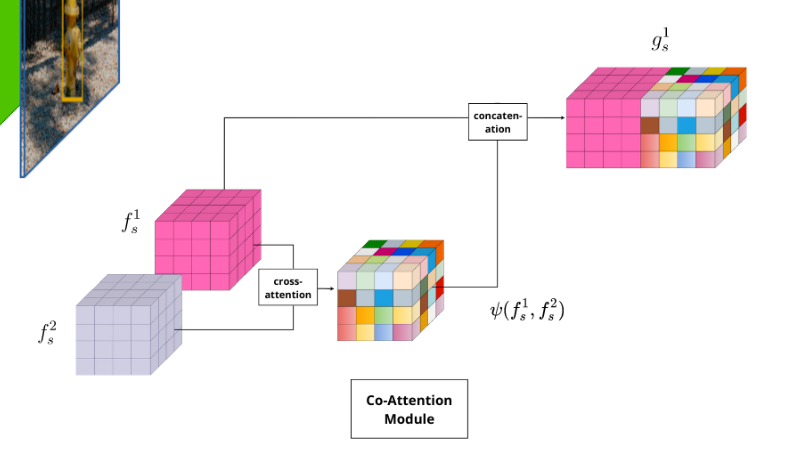
\includegraphics[width=\linewidth]{Co_Attention_Module.png}
    \end{figure}
\end{frame}
%------------------------------------------------

\begin{frame}
    \onehalfspacing
        \frametitle{Use Siamese network to detect changes}
            \begin{figure}[h]
                \centering
                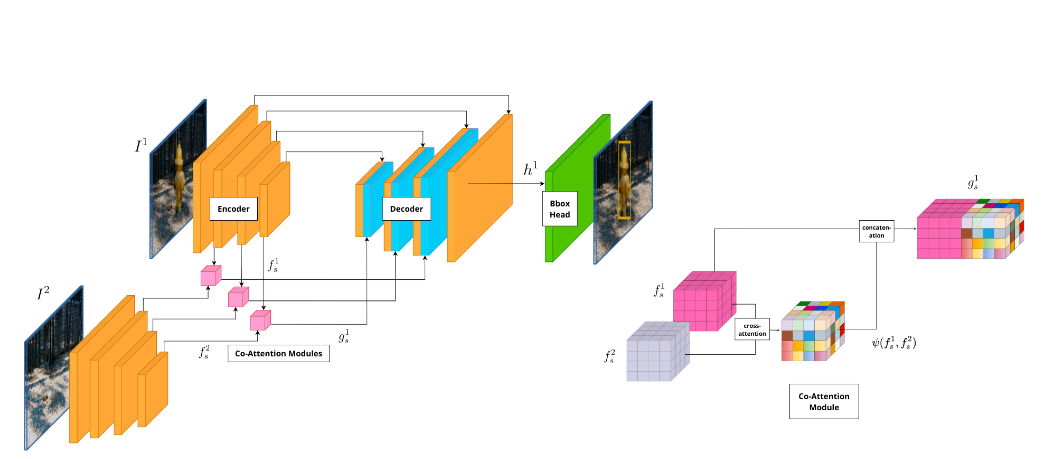
\includegraphics[scale=0.4]{Siamese_network_architecture.png}
            \end{figure}
        
            \begin{itemize}
                \item First obtaining a set of dense feature
                descriptors for each image using a CNN-based (ResNet50) encoder.
                \item These feature are then conditioned on
                each other using a co-attention mechanism that implicitly
                supplies the correspondences.

            \end{itemize}
    \end{frame}
    %------------------------------------------------


\begin{frame}
    \onehalfspacing
        \frametitle{Use Siamese network to detect changes}
            \begin{figure}[h]
                \centering
                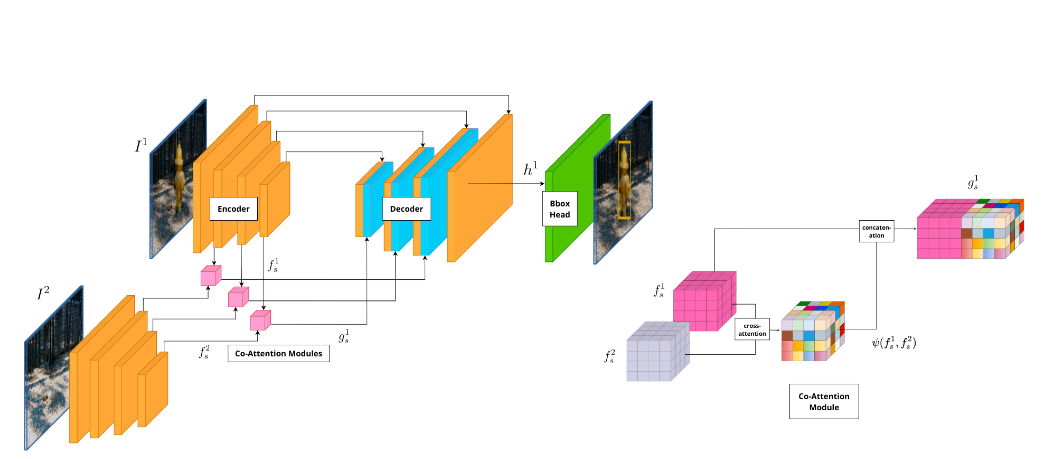
\includegraphics[scale=0.4]{Siamese_network_architecture.png}
            \end{figure}
        
            \begin{itemize}
                \item Next, feature are passed through a decoder to obtain high
                resolution conditioned image descriptors which are used
                by a bounding box detection head to localise the changes.
            \end{itemize}
    \end{frame}
    %------------------------------------------------


\begin{frame}
    \onehalfspacing
        \frametitle{Siamese Network: Dataset}
        For this method, we make use of a state-of-the-art image inpainting method, \textbf{LaMa}, to make the objects \textit{disappear}. 
        \begin{figure}[h]
            \centering
            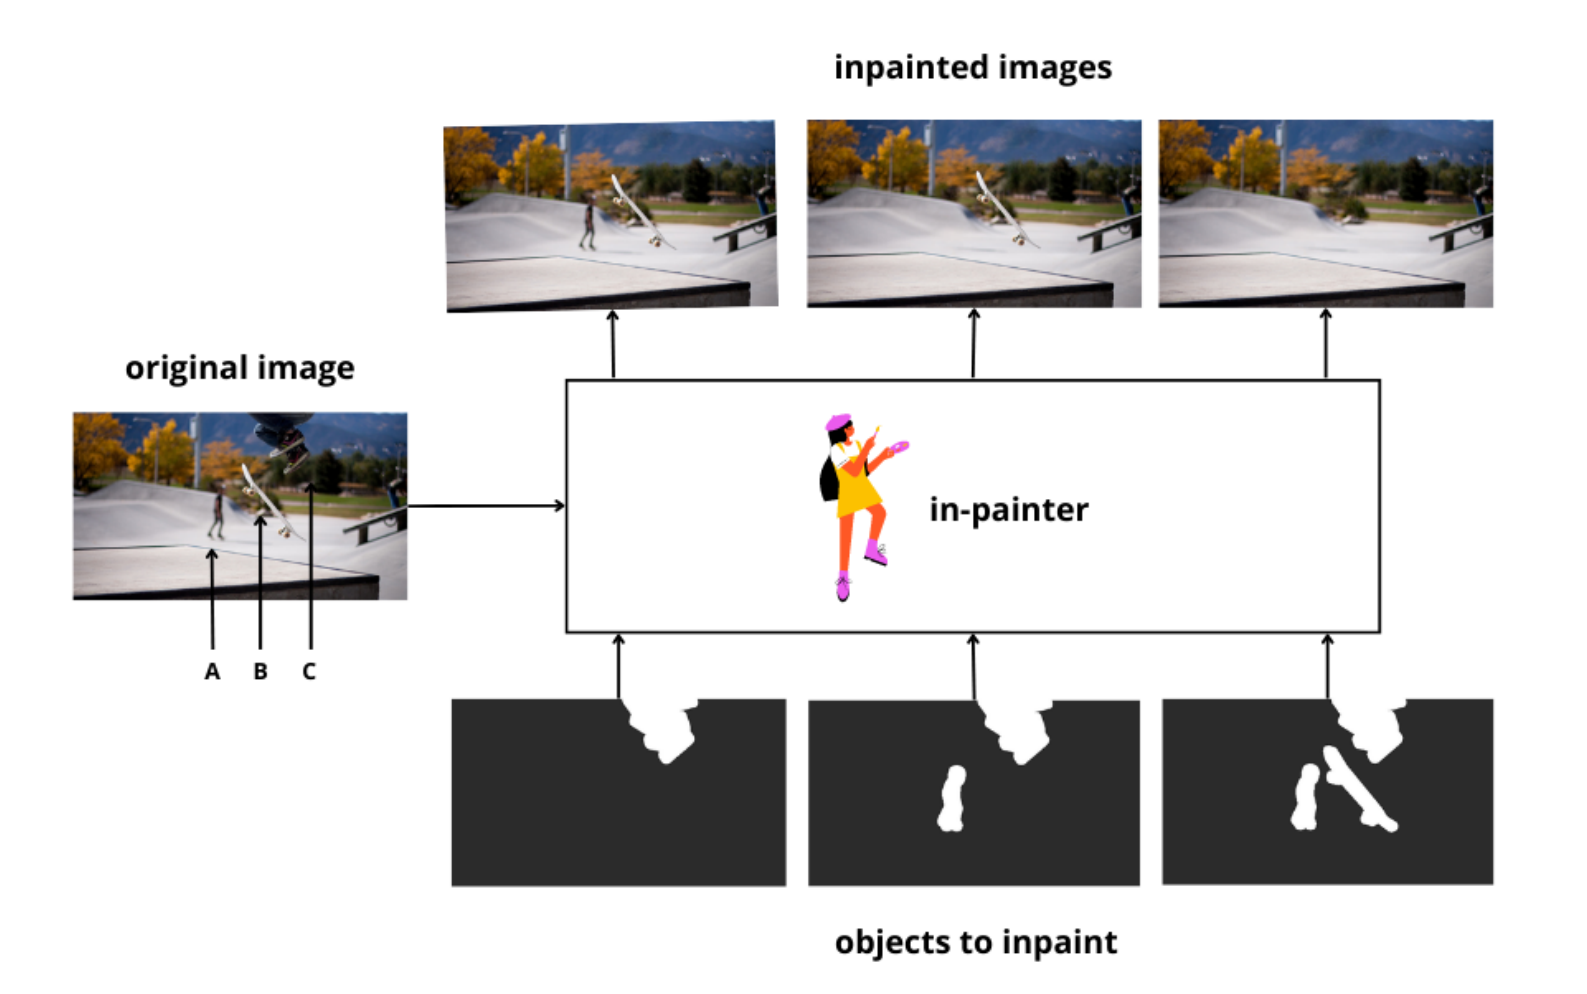
\includegraphics[width=\linewidth]{Lama.png}
        \end{figure}
    \end{frame}
%------------------------------------------------
\begin{frame}
    \onehalfspacing
        \frametitle{Siamese Network: Dataset}
       
            \begin{itemize}
                \item We also apply random affine transformations to the images along with colour jittering or add random text to “background” images.
                \item Datasets: COCO-Inpainted, Synthtext-Change, VIRAT-STD, Kubric-Change.
                
            \end{itemize}

            \begin{figure}[h]
                \centering
                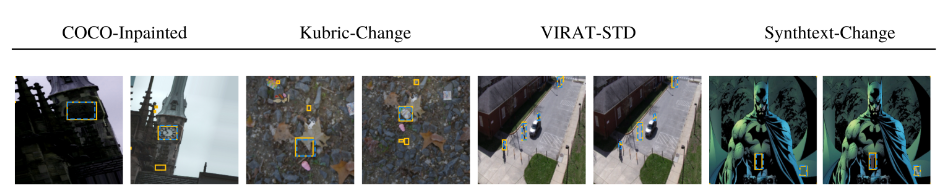
\includegraphics[width=\linewidth]{Siamese_dataset.png}
            \end{figure}

    \end{frame}

%------------------------------------------------
\section{Experiments}

\begin{frame}
    \doublespacing
        \frametitle{Presentation Overview} % Slide title, remove this command for no title
        
        \tableofcontents[currentsection] % Output the table of contents (all sections on one slide)
        %\tableofcontents[pausesections] % Output the table of contents (break sections up across separate slides)
\end{frame}

%------------------------------------------------

\begin{frame}
    \onehalfspacing
        \frametitle{VIRAT Video Dataset}
       
        \begin{block}{VIRAT Video Dataset}
            A large-scale surveillance video dataset includes videos collected from
            stationary ground cameras and aerial vehicles. It has several event types:
        
            \begin{itemize}
                \item \textbf{Single Person Events} (8): walking, running, standing,
                throwing, gesturing, carrying, loitering, picking up
                \item \textbf{Person and Vehicle Events} (7): getting into or out of
                vehicle, opening or closing trunk, loading, unloading, dropping off, bicycling
                \item \textbf{Person and Facility Events} (2): entering or exiting facility
            \end{itemize}
        \end{block}
            \begin{figure}[h]
                \centering
                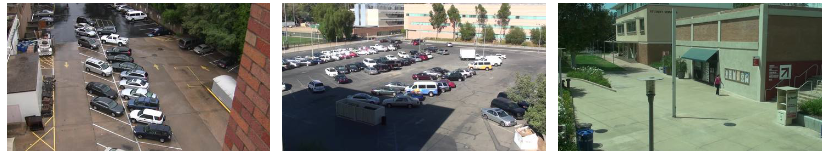
\includegraphics[width=\linewidth]{VIRAT_datasets.png}
            \end{figure}

    \end{frame}

%------------------------------------------------

\begin{frame}
    \onehalfspacing
        \frametitle{ Evaluation Metrics}
       
        \begin{block}{}
            To assess the effectiveness of the proposed methods, we will employ key performance metrics: \textit{precision, recall, and F1 score}. 
        \end{block}

        We calculate these metrics for a set of ground truth and predicted bounding boxes corresponding to specific
        image.

        \begin{table}[htbp]
            \centering
            \caption{Performance Evaluation of Different Approaches}
            \label{tab:performance}
            \begin{tabular}{lccc}
                \toprule
                \textbf{Approach} & \textbf{Precision} & \textbf{Recall} & \textbf{F1 Score} \\
                \midrule
                Pixel-wise & .354 & . 584 & .441 \\
                SSIM & .314 & .169 & .22 \\
                Siamese Network & .354 & .584 & .441 \\
                \bottomrule
            \end{tabular}
        \end{table}
    \end{frame}

%------------------------------------------------

\begin{frame}
    \onehalfspacing
        \frametitle{Output Examples: Siamese Network}    
        \begin{figure}
            \begin{subfigure}{0.5\textwidth}
              \centering
              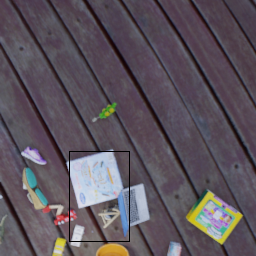
\includegraphics[width=\linewidth]{Example/Output/SM_2.png}
              \captionsetup{labelformat=empty}
            \end{subfigure}%
            \begin{subfigure}{0.5\textwidth}
              \centering
              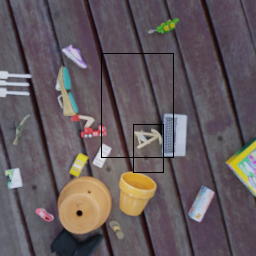
\includegraphics[width=\linewidth]{Example/Output/SM_2_2.png}
              \captionsetup{labelformat=empty}
            \end{subfigure}
            \captionsetup{labelformat=empty}
        \end{figure}

    \end{frame}

%------------------------------------------------

\begin{frame}
    \onehalfspacing
        \frametitle{Output Examples: Siamese Network}    
        \begin{figure}
            \begin{subfigure}{0.5\textwidth}
              \centering
              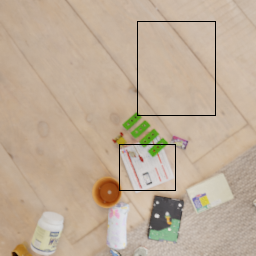
\includegraphics[width=\linewidth]{Example/Output/SM_1.png}
              \captionsetup{labelformat=empty}
            \end{subfigure}%
            \begin{subfigure}{0.5\textwidth}
              \centering
              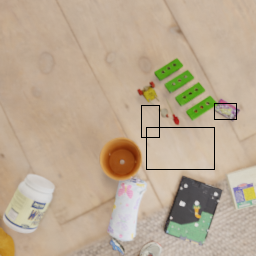
\includegraphics[width=\linewidth]{Example/Output/SM_1_2.png}
              \captionsetup{labelformat=empty}
            \end{subfigure}
            \captionsetup{labelformat=empty}
        \end{figure}

    \end{frame}

%------------------------------------------------

\begin{frame}
    \onehalfspacing
        \frametitle{Output Examples: Siamese Network}    
        \begin{figure}
            \begin{subfigure}{0.5\textwidth}
              \centering
              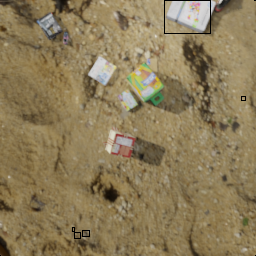
\includegraphics[width=\linewidth]{Example/Output/SM_3.png}
              \captionsetup{labelformat=empty}
            \end{subfigure}%
            \begin{subfigure}{0.5\textwidth}
              \centering
              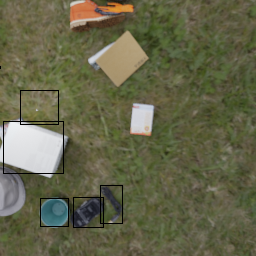
\includegraphics[width=\linewidth]{Example/Output/SM_3_2.png}
              \captionsetup{labelformat=empty}
            \end{subfigure}
            \captionsetup{labelformat=empty}
        \end{figure}

    \end{frame}

%------------------------------------------------


\begin{frame}
    \onehalfspacing
        \frametitle{Output Examples: SSIM}    
        \begin{figure}
            \begin{subfigure}{0.5\textwidth}
              \centering
              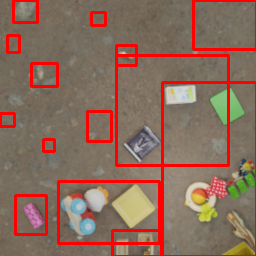
\includegraphics[width=\linewidth]{Example/Output/SSIM_1.png}
              \captionsetup{labelformat=empty}
            \end{subfigure}%
            \begin{subfigure}{0.5\textwidth}
              \centering
              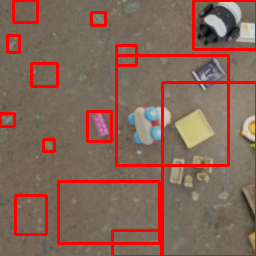
\includegraphics[width=\linewidth]{Example/Output/SSIM_1_2.png}
              \captionsetup{labelformat=empty}
            \end{subfigure}
            \captionsetup{labelformat=empty}
        \end{figure}

    \end{frame}

%------------------------------------------------

\begin{frame}
    \onehalfspacing
        \frametitle{Output Examples: Pixel-wise}    
        \begin{figure}
            \begin{subfigure}{0.5\textwidth}
              \centering
              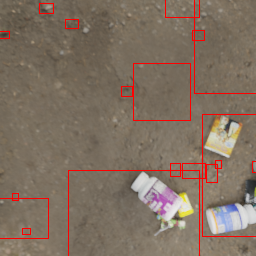
\includegraphics[width=\linewidth]{Example/Output/PW_1.png}
              \captionsetup{labelformat=empty}
            \end{subfigure}%
            \begin{subfigure}{0.5\textwidth}
              \centering
              \includegraphics[width=\linewidth]{Example/Output/PW_1_2.png}
              \captionsetup{labelformat=empty}
            \end{subfigure}
            \captionsetup{labelformat=empty}
        \end{figure}

    \end{frame}

%------------------------------------------------





\onehalfspacing
\begin{frame} % Use [allowframebreaks] to allow automatic splitting across slides if the content is too long
	\frametitle{Reference}
	
	\begin{thebibliography}{99} % Beamer does not support BibTeX so references must be inserted manually as below, you may need to use multiple columns and/or reduce the font size further if you have many references
		\footnotesize % Reduce the font size in the bibliography
		
		\bibitem[Stanford]{p1}
			\href{https://arxiv.org/pdf/2209.14341.pdf}{The Change You Want To See}
			\newblock Ragav Sachdeva and Andrew Zisserman

        \bibitem[Stanford]{p2}
        \href{https://www.cns.nyu.edu/pub/eero/wang03-reprint.pdf}{Image Quality Assessment: From Error Visibility to
        Structural Similarity}
			\newblock Zhou Wang, Alan Conrad Bovik, Hamid Rahim Sheikh and Eero P. Simoncelli
		
        \hspace{-1.9em}\includegraphics[width=1.5em]{Icons/github.png}
        \textcolor{blue}{\href{https://github.com/ragavsachdeva/The-Change-You-Want-to-See/tree/main?fbclid=IwAR0LKUHmVIEYSDTCgl2KeV5jir1pUlMSYJTbHbirilqWH_eZ4N9FxHwTQto\#datasets}{Datasets: The Change You Want to See (WACV 2023).}}
          \newblock \textcolor{black}{Ragav Sachdeva and Andrew Zisserman}
	\end{thebibliography}
\end{frame}



%	CLOSING SLIDE
%----------------------------------------------------------------------------------------

\begin{frame} % The optional argument 'plain' hides the headline and footline
	\begin{center}
		{\Huge Thanks for listening!}
		
		\bigskip\bigskip % Vertical whitespace
		
		{\LARGE Q\&A section}
	\end{center}
\end{frame}
%------------------------------------------------


\end{document}
